
Expectation maximization (EM) algorithm is a general
method for finding ML and MAP estimates in probabilistic models with missing data or
latent variables. It was first introduced in
the celebrated article of \textcite{Dempster1977}. Instead of maximizing
\eqref{eq:logLH} directly, EM alternates between computing a variational lower bound and then maximizing this bound
\parencite{Bishop2006,barber2012bayesian}. As will be seen, since the bound is strict, increasing the bound implies
an increase in the objective function. For these reasons EM is well described as lower bound optimization \parencite{Minka1998}.
We shall use $\E{\cdot}_{q}\equiv\defint{}{}{\cdot\,\Pdf[q]{z}}{z}$ to denote the expectation
over any distribution $\Pdf[q]{z}$.

Let us introduce a family of ``variational'' distributions 
indexed by the parameter $\gv{\psi}$, $\tPX$, over the states $\X$ (or the latent variables in general).
Noting now that $\Pdf{\X}{\Y,\Th}=\cLH/\LH$ and that $\lLH\equiv\log\LH$ is independent of $\X$ we can then perform the
following decomposition on the log likelihood:
\begin{align}
	\lLH &= \log\cLH - \log\post \nonumber\\
	&= \E{\log\cLH}_{\tPX} - \E{\log\post}_{\tPX} \nonumber\\ 
	\begin{split}
	&=\underbrace{\E{\log\cLH}_{\tPX} - \E{\tPX}_{\tPX}}_{\displaystyle \EMB{\gv{\psi}}{\Th}}\\
	&\quad+\KL{\tPX}{\post}. 
	\end{split}
	\label{eq:lLH_decomp}
\end{align}
By invoking the nonnegativeness of
the \emph{Kullback-Leibler divergence}
\begin{align}
		\KL{\tPX}{\post} = -\E{\log{\frac{\post}{\tPX}}}_{\tPX},  
\end{align}
or equivalently the relation
\begin{align}
	\E{\log\tPX}_{\tPX} &\geq \E{\log\post}_{\tPX},	
\end{align}
provable by \emph{Jensen's inequality}, 
we see that $\EMB{\gv{\psi}}{\Th}$ is indeed a lower bound on $\lLH$. 
These considerations suggest an iterative algorithm
which produces a series of estimates $\brac{\Th_j}$, where $j=0,\dots$.
Given the initial guess $\Th_0$, the two alternating
steps of the algorithm are:
%
\begin{description}
\addtolength{\leftskip}{1cm}
  \item[E-step]\hfill\\
  Set $\tPX{\gv{\psi}_{j+1}}$ to the distribution that maximizes $\EMB{\gv{\psi}}{\Th_j}$
  with respect to $\gv{\psi}$. Here $\Th_j$ is the current estimate of $\Th$.  
  \item[M-step]\hfill\\ 
  Set $\Th_{j+1}$ to the estimate that maximizes $\EMB{\gv{\psi}_{j+1}}{\Th}$ with respect to $\Th$.
\end{description}%
In some sense then, the algorithm can be viewed as coordinate ascent in $\EMB{\gv{\psi}}{\Th}$ \parencite{Neala1998}. 

The \emph{sharpest} bound can clearly be found among
distributions of the form $\post{\Th'}$, since the Kullback-Leibler divergence 
vanishes with $\tPX= \post$.
Let us now define
\begin{align}
	\EMQ &\equiv \E{\log\cLH}_{\post{\Th'}} \label{eq:EM_Q}\\
	\EMH &\equiv \E{\log\post}_{\post{\Th'}} \label{eq:EM_H}\\
	\EMB &\equiv \EMQ - \EMH{\Th'}{\Th'} \label{eq:EM_B}.
\end{align}
Regarding these functions we will use the convention that denoting for example $\EMB{\gv{\psi}}{\Th}$ means the
expectation is taken with respect to some \emph{unspecified} distribution $\tPX$, whereas $\EMB$ implies
that it is taken with respect to the posterior distribution of the states with parameter $\Th'$, i.e. $\post{\Th'}$. 


According to \eqref{eq:lLH_decomp} we now have
\begin{align}
	\lLH & \geq \EMB \quad \forall \Th,\Th' \in \Theta
	\label{eq:EM_LB}
\end{align}
and especially
\begin{align}
	\lLH & = \EMB{\Th}{\Th}.
	\label{eq:EM_sharp_bound}
\end{align}
When we want to maximize $\EMB$ with respect to $\Th$
clearly it suffices to consider
only $\EMQ$, known as the \emph{expected complete-data log-likelihood}
or the \emph{intermediate quantity of EM} \parencite{Cappe2005,Bishop2006}.

What is also interesting about $\EMQ$ is that it can be used to compute the gradient of the log-likelihood, i.e
the score, itself. From equations \eqref{eq:EM_B}
and \eqref{eq:EM_sharp_bound} it can be seen rather easily, that  
the score evaluated at $\widehat{\Th}$ is given by
\begin{align}
		\score[\widehat\Th]&=
		\nabla_{\Th}\EMQ[\big]{\widehat\Th}{\widehat\Th}
		\equiv\eval{\dpd{ \EMQ[\big]{\widehat\Th}{\Th}}{\Th}}_{\Th=\widehat\Th} \label{eq:EM_gradients}
\end{align} 
Equation \eqref{eq:EM_gradients} is known as \emph{Fisher's identity} \parencite{Cappe2005}. It gives
an alternative route for the score function computation.
The implications will be discussed in more detail in the sequel.

We are now in a position to formulate the so called \emph{fundamental inequality of EM} \parencite{Cappe2005}.
From \eqref{eq:EM_LB} we have
\begin{align*}
	\lLH[\Th_{j+1}] & \geq \EMQ{\Th_j}{\Th_{j+1}} - \EMH{\Th_j}{\Th_{j}},
\end{align*}
so that using \eqref{eq:EM_sharp_bound} and assuming that the M-step result $\Th_{j+1}$ increases
the bound we can write
\begin{align}
\label{eq:fundamental_inequality}	
\begin{split}	
	\lLH[\Th_{j+1}] - \lLH[\Th_j] & \geq \EMQ{\Th_j}{\Th_{j+1}} - \EMQ{\Th_j}{\Th_{j}} \geq 0\\
\end{split}
\end{align}
This highlights
the fact that \emph{the likelihood is increased or unchanged with every new estimate} $\Th_{j+1}$.
Also following from \eqref{eq:fundamental_inequality} is the fact that if the iterations
stop at a certain point, i.e. $\Th_{l}=\Th_{l-1}$ at iteration $l$, then
$\EMQ{\Th_l}{\Th}$ must be maximal at $\Th=\Th_l$ and thus its gradient, and 
by \eqref{eq:EM_gradients} that of the likelihood, must be zero at $\Th=\Th_l$. Thus
$\Th_l$ is a \emph{stationary point} of $\lLH$, i.e a local maximum or a saddle point.

Figure~\ref{fig:ar1_em} illustrates the EM algorithm for a unidimensional parameter 
$\theta$. Starting from the lower left corner, given the current parameter estimate
$\theta_k$, the E-step computes the lower bound $\EMB{\theta_k}{\theta}$ (dashed line) 
to the objective function $\lLH[\theta]$ (solid line). Clearly $\EMB{\theta_k}{\theta_k}=\lLH[\theta_k]$
and $\nabla_{\theta}\EMB{\theta_k}{\theta_k}=\nabla_{\theta}\EMQ{\theta_k}{\theta_k}=\score[\theta_k]$.
In the M-step, the next parameter value $\theta_{k+1}$ is found by maximizing the lower bound obtained
in the E-step. In the case of Figure~\ref{fig:ar1_em}, we can see that EM estimate is very close
to the ML estimate at iteration $k+2$. 

\begin{figure}[htb]%
    \centering%
  	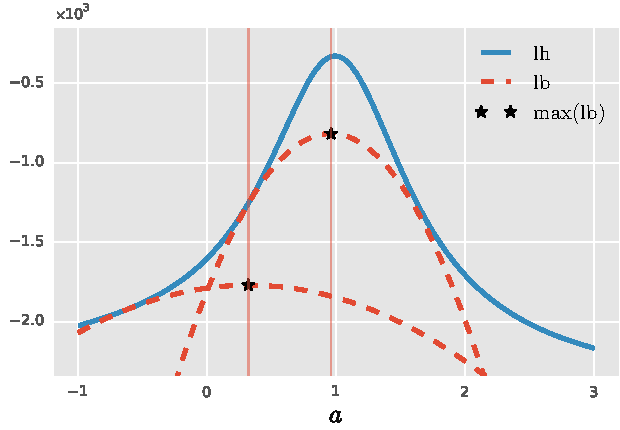
\includegraphics{img/ar1_ex_em}%
	\caption{%
Illustration of two iterations of the EM algorithm for a unidimensional parameter 
$\theta$. Starting from the lower left corner, given the current parameter estimate
$\theta_k$, the E-step computes the lower bound (dashed line) 
to the objective function $\lLH[\theta]$ (solid line). In the M-step, the next parameter 
value $\theta_{k+1}$ is found by maximizing the lower bound obtained in the E-step. The 
EM estimate is very close to the ML estimate at iteration $k+2$.
   	}
	\label{fig:ar1_em}
 \end{figure}

We have so far formulated the EM algorithm only for ML estimation. In case
of MAP estimation with nonuniform prior (remember that with a uniform prior the estimates are identical), 
the E-step stays the same since the prior is independent of $\X$.
The MAP M-step is
\begin{description}
\addtolength{\leftskip}{1cm}
  \item[M-step (MAP)]\hfill\\ 
  Set $\Th_{j+1}$ to the estimate that maximizes $\EMB{\gv{\psi}_{j+1}}{\Th}+\log\Pdf{\Th}$ with respect to $\Th$.
\end{description}%


 

%%%%%%%%%%%%%%%%%%%%%%%%%%%%%%%%%%%%%%%%%%%%%%%%%%%%%%%%%%%%%%%%%%%%%%%%%%%%%%%%%%
\subsubsection*{EM in exponential families of distributions}\label{sec:EM_exp}%
%%%%%%%%%%%%%%%%%%%%%%%%%%%%%%%%%%%%%%%%%%%%%%%%%%%%%%%%%%%%%%%%%%%%%%%%%%%%%%%%%%

Computing the intermediate quantity of EM is especially simple
if the dynamic model and the measurement model belong to an exponential
family of distributions, which have probability distribution functions of the form 
\begin{align}
	\Pdf[q]{\z}{\Th}&=\F{h}{\z}\exp\brac[\big]{ \F{\gv{\psi}}{\Th}^\tr \F*{s}{\z}-\F{c}{\Th}}.
	\label{eq:exp_family}
\end{align}
Here $\F*{s}{\z}$ is called the vector of \emph{natural sufficient statistics} and
$\gv{\eta}\equiv \F{\gv{\psi}}{\Th}$ is the \emph{natural parameterization}.
Let us suppose now that the complete-data likelihood is of the form \eqref{eq:exp_family}, so
that $\v{z}^\tr=\brak*{\mathrm{vec}\brac*{\X}^\tr,\mathrm{vec}\brac*{\Y}^\tr}$, where the operator $\mathrm{vec}\brac*{\cdot}$
creates vectors out of matrices by stacking their columns. Thus $\v{z}$ 
contains the hidden variables $\X$ and the measurements $\Y$. 

The intermediate quantity, i.e the expectation of the logarithm of $\Pdf[q]{\z}{\Th}$ over the posterior distribution of 
$\X$ (implicit in the notation) becomes now
\begin{align}
	\EMQ&=	\F{\gv{\psi}}{\Th}^\tr \E{\F*{s}{\z}}-\F{c}{\Th}+\E{\F{h}{\z}}.
\end{align}
Since the last term is independent of $\Th$ then the maximization in the M-step
is independent of this last term. Thus the role of the E-step degenerates into computing the
expectation of the sufficient statistics $\E{\F*{s}{\z}}$.



%%%%%%%%%%%%%%%%%%%%%%%%%%%%%%%%%%%%%%%%%%%%%%%%%%%%%%%%%%%%%%%%%%
\subsubsection*{EM as a special case of variational Bayes}%%%%%%
%%%%%%%%%%%%%%%%%%%%%%%%%%%%%%%%%%%%%%%%%%%%%%%%%%%%%%%%%%%%%%%%%%


Variational Bayes (VB) is a fully Bayesian methodology where one seeks
for an approximation to the parameter posterior \parencite{barber2012bayesian,Bishop2006,Mackay2004,beal2003variational}
\begin{align}
	\Pdf{\Th}{\Y} &= \frac{1}{Z}\Pdf{\Y}{\Th}\Pdf{\Th} \approx \Pdf[q]{\Th}. 
\end{align}
Let us introduce the following simplifying
factorization to the joint posterior of states and parameters.
\begin{align}
	\Pdf{\X,\Th}{\Y}\approx \Pdf[q]{\X}\Pdf[q]{\Th}
	\label{eq:VB_factorization}
\end{align}
Noting now that $\Pdf{\X,\Th}{\Y}=\Pdf{\X,\Y,\Th}/\LH$ and that $\lLH\equiv\log\LH$ is independent of $\X$ we can then perform the
following decomposition on the log likelihood:
\begin{align}
	\lLH &= \log\Pdf{\X,\Y,\Th} - \log\Pdf{\X,\Th}{\Y} \nonumber\\
	&= \E{\log\Pdf{\X,\Y,\Th}}_{\Pdf[q]{\X}\Pdf[q]{\Th}} - \E{\Pdf{\X,\Th}{\Y}}_{\Pdf[q]{\X}\Pdf[q]{\Th}} \nonumber\\ 
	\begin{split}
	&=\E{\log\Pdf{\X,\Y,\Th}}_{\Pdf[q]{\X}\Pdf[q]{\Th}} -  \E{\Pdf[q]{\X}}_{\Pdf[q]{\X}} - \E{\Pdf[q]{\Th}}_{\Pdf[q]{\Th}}\\
	&\quad+\KL{\Pdf[q]{\X}\Pdf[q]{\Th}}{\Pdf{\X,\Th}{\Y}}. 
	\end{split}
	\label{eq:lLH_decomp_vb}
\end{align}
Thus minimizing the KL divergence between the factorized approximation and the true joint posterior is equivalent to finding the tightest lower bound to
the log likelihood. 
These considerations suggest an iterative algorithm
which produces a series of estimates $\Pdf[q_j]{\Th}$, where $j=0,\dots$.
Given the initial guess $\Pdf[q_0]{\Th}$, the two alternating
steps of the algorithm are:

\begin{description}
\addtolength{\leftskip}{1cm}
\item[E-step]
\begin{align}
	\Pdf[q_{j+1}]{\X}=\argmin_{\Pdf[q]{\X}}\KL{\Pdf[q]{\X}\Pdf[q_{j}]{\Th}}{\Pdf{\X,\Th}{\Y}}
	\label{eq:VB_E}
\end{align}
\item[M-step]
\begin{align}
	\Pdf[q_{j+1}]{\Th}=\argmin_{\Pdf[q]{\Th}}\KL{\Pdf[q_{j+1}]{\X}\Pdf[q]{\Th}}{\Pdf{\X,\Th}{\Y}}
	\label{eq:VB_M}
\end{align}
\end{description}

Let us then suppose that we only wish to find the MAP point estimate $\Th^*$. This can be accomplished
by assuming a delta function form $\Pdf[q]{\Th}=\delta\left(\Th,\Th^*\right)$ for the parameter factor in the
joint distribution of states and parameters \eqref{eq:VB_factorization}.
With this assumption equation the bound becomes
\begin{align}
	\Pdf{\Y}{\Th^*} &\geq \E{\Pdf{\X,\Th^*,\Y}}{\Pdf[q]{\X}\Pdf[q]{\Th}} - \E{\Pdf[q]{\X}}{\Pdf[q]{\X}} + \mathtt{const}
	\label{eq:VB_MAP_boundl}
\end{align}
and the ``M''-step \eqref{eq:VB_M} can then be written as
\begin{align}
	\Th_{j+1} &= \argmax_{\Th}\brak*{\E{\log\cLH}{\Pdf[q]{\X}}+\log\Pdf{\Th}}.	
\end{align}
If the point estimate is plugged in the ``E''-step equation \eqref{eq:VB_E} we have
\begin{align}
	\Pdf[q_{j+1}]{\X}\propto \Pdf{\X,\Y}{\Th_j} \propto \Pdf{\X}{\Y,\Th_j} 	
\end{align}
Thus the EM algorithm can deduced to be a special case of VB with a delta function form
of $\Pdf[q]{\Th}$.


%%%%%%%%%%%%%%%%%%%%%%%%%%%%%%%%%%%%%%%%%%%%%%%%%
\subsubsection{Partial E and M steps}%%%%%%%%%%
%%%%%%%%%%%%%%%%%%%%%%%%%%%%%%%%%%%%%%%%%%%%%%%%%
\label{sec:EM_partial}
As can be seen from equation~\eqref{eq:fundamental_inequality},
to ensure monotonicity it is enough that $\EMQ{\Th_j}{\Th_{j+1}}\geq \EMQ{\Th_{j}}{\Th_j}$,
i.e. $\Th_{j+1}$ is not required to be the maximum of $\EMQ{\Th_j}{\Th}$.
This was observed already in \textcite{Dempster1977}, where methods
that only seek an increase in the M-step were termed 
\emph{generalized} EM (gEM) algorithms. 

Another modification is the partial, or approximate, E-step. It is clear
that in this case, i.e. when we cannot compute $\post$ exactly, the Kullback-Leibler 
divergence in decomposition \eqref{eq:lLH_decomp} is strictly positive. This
means that the lower bound we are optimizing never ``touches'' the log-likelihood
as in equation \eqref{eq:EM_sharp_bound} and Figure~\ref{fig:ar1_em}. 
Thus EM with an approximate  E step is not an ascent 
algorithm anymore \parencite{Goodwin2005}.

% When we restrict the approximation $\tPX$ to $\post$ to a certain
% family of probability distribution and choose the one which
% minimizes $\KL{\tPX}{\post}$, the resulting algorithm is known
% as \emph{variational Expectation Maximization} (vEM) \parencite{Turner2011}.
% When we restrict $\tPX$ to be Gaussian via moment matching, as is the case
% in Gaussian filtering/smoothing, this KL divergence is in fact minimized.
% Suppose now that $\gv{\psi}\equiv \brac{\m,\P}$, where $\m$ is the mean and \todo{fill up the moment matching KL equations}
% $\P$ is the covariance matrix. Then
% \begin{align}
% 	\dpd{}{\m}\KL{\tPX}{\post} &= \\
% 	\dpd{}{\P}\KL{\tPX}{\post} &=.
% \end{align}
% Setting these simultaneously to zero we obtain
% \begin{align}
% 	\dpd{\KL{\tPX}{\post}}{\m} &= \\
% 	\dpd{\KL{\tPX}{\post}}{\P} &=
% \end{align}


%%%%%%%%%%%%%%%%%%%%%%%%%%%%%%%%%%%%%%%%%%%%%%%%
\subsubsection{Linear-Gaussian SSMs}%%%%%%%%%%
%%%%%%%%%%%%%%%%%%%%%%%%%%%%%%%%%%%%%%%%%%%%%%%%
\label{sec:EM_SSM}

Let us then turn to applying EM to the case of linear-Gaussian SSMs
\parencite{shumway1982approach,Ghahramani1996}
, so that
\begin{align}
	\ff &\equiv \v{A}\xkk\\
	\hh &\equiv \v{H}\xk\\
	\Th &\equiv \brac{\v{A},\v{Q},\v{H},\v{R}}.
	\label{tablelabel}
\end{align}
First of all, from the factorization in \eqref{eq:complete_data_likelihood}, the complete-data log-likelihood becomes
\begin{align}
\label{eq:clLH_LG}
\begin{split}
	\lLH
	=&-\frac{1}{2}\left(\x_0-\gv{\mu}_0\right)^\tr\gv{\Sigma}_0^{-1}\left(\x_0-\gv{\mu}_0\right)-\frac{1}{2}\log\detr{\gv{\Sigma}_0}\\
	&-\frac{1}{2}\sum_{k=1}^T\left(\x_k-\v{A}\xkk\right)^\tr\v{Q}^{-1}\left(\x_k-\v{A}\xkk)\right)-\frac{T}{2}\log\detr{\v{Q}}\\
	&-\frac{1}{2}\sum_{k=1}^T\left(\y_k-\v{H}\xk\right)^\tr\v{R}^{-1}\left(\y_k-\v{H}\xk\right)-\frac{T}{2}\log\detr{\v{R}}\\
	&+\mathtt{const}
\end{split}
\end{align}
Taking the expectation of \eqref{eq:clLH_LG} with respect to $\Pdf{\X}{\Y,\Th'}$ (assumed implicitly in the notation),
applying the identity $\v{a}^\tr\v{C}\v{b}=\Tr{\v{a}^\tr\v{C}\v{b}}=\Tr{\v{C}\v{b}\v{a}^\tr}$, and dropping the constant terms we get
\begin{align}
\begin{split}
	\EMQ{\Th'}{\Th} \approx -\frac{1}{2}\bigg\{&\Tr{\gv{\Sigma}_0^{-1}\E{\left(\x_0-\gv{\mu}_0\right)\left(\x_0-\gv{\mu}_0\right)^\tr}}+\log\detr{\gv{\Sigma}_0}\\
	+\,&\Tr[\bigg]{\v{Q}^{-1}\sum_{k=1}^T\E{\left(\x_k-\v{A}\xkk\right)\left(\x_k-\v{A}\xkk\right)^\tr}}+T\log\detr{\v{Q}}\\
	+\,&\Tr[\bigg]{\v{R}^{-1}\sum_{k=1}^T\E{\left(\y_k-\v{H}\xk\right)\left(\y_k-\v{H}\xk\right)^\tr}}+T\log\detr{\v{R}}\bigg\}
\end{split}
\label{eq:eclLH}
\end{align} 
Let us denote the terms inside the traces in equation~\eqref{eq:eclLH} with
\begin{align}
	\II{1} &= \E{\left(\x_0-\gv{\mu}_0\right)\left(\x_0-\gv{\mu}_0\right)^\tr}\\ 
	&=\defint{\mathcal{X}\times T}{}{\left(\x_0-\gv{\mu}_0\right)\left(\x_0-\gv{\mu}_0\right)^\tr\Pdf{\X}{\Y,\Th'}}{\X}\nonumber\\
	&= 	\defint{\mathcal{X}}{}{\left(\x_0-\gv{\mu}_0\right)\left(\x_0-\gv{\mu}_0\right)^\tr\Pdf{\x_0}{\Y,\Th'}}{\x_0} \label{eq:I1_general}\\
	\II{2} &= \sum_{k=1}^T\defint{\mathcal{X}}{}{\left(\x_k-\v{A}\xkk\right)\left(\x_k-\v{A}\xkk\right)^\tr\Pdf{\xk,\xkk}{\Y,\Th'}}{\xk}{\xkk} \label{eq:I2_general}\\
	\II{3} &=
	\sum_{k=1}^T\defint{\mathcal{X}}{}{\left(\y_k-\v{H}\xk\right)\left(\y_k-\v{H}\xk\right)^\tr\Pdf{\xk}{\Y,\Th'}}{\xk}
	\label{eq:I3_general} \end{align}%
%
%
It is clear then that in the E-step one needs to compute the $T+1$ smoothing
distributions, including the $T$ cross-timestep distributions, since these
will be needed in the expectations.
By applying the identity
\begin{align}
	\var{\x}&=\E{\x\x^\tr}-\E{\x}\E{\x}^\tr,
\end{align} 
we can write first expectation as
\begin{align}
	\II{1}&= \v{P}_{0|T}+(\v{m}_{0|T}-\gv{\mu}_0)(\v{m}_{0|T}-\gv{\mu}_0)^\tr,
	\label{eq:I1}
\end{align}
where we denote Gaussian smoothing distributions by $\Pdf{\xk}{\Y}=\N[\xk]{\m_{k|T}}{\P_{k|T}}$.
This was a result of assuming the Gaussian prior distribution of equation~\eqref{eq:prior} and
it is common for the more specific models we're assessing in the next chapters.

As in \eqref{eq:joint_smoothing}, let us also denote the joint smoothing distribution of $\xk$ and $\xkk$ by
\begin{align}
\Pdf{\xkk,\xk}{\Y}&=\N[\bm{\xkk\\\xk}]{
	\bm{
		\m_{k-1|T}\\
		\m_{k|T}
	}}{
	\bm{
		\P_{k-1|T}&\v{D}_{k-1}\\
		\v{D}_{k-1}^\tr&\P_{k|T}
	}}
	\label{eq:pdf_smooth_joint}.
\end{align}
Then by applying the manipulation
\begin{align}
\begin{split}
&\E{\left(\v{A}\v{x}_{k-1}-\v{x}_k\right)\left(\v{A}\v{x}_{k-1}-\v{x}_k\right)^\tr}\\
=&\bm{\v{A}^\tr \\ -\v{I}}^\tr	
\E{
\begin{bmatrix}
	\xkk\\\xk
\end{bmatrix}
\begin{bmatrix}
	\xkk \\ \xk	
\end{bmatrix}^\tr
}
\bm{\v{A}^\tr\\-\v{I}}	
\end{split}
\end{align}
we get
\begin{align}
	\II{2}&=
\bm{\v{A}^\tr \\ -\v{I}}^\tr	
\sum_{k=1}^T\left(\bm{
		\P_{k-1|T}&\v{D}_{k-1}\\
		\v{D}_{k-1}^\tr&\P_{k|T}
	}+\bm{
		\m_{k-1|T}\\
		\m_{k|T}
	}\bm{
		\m_{k-1|T}\\
		\m_{k|T}
	}^\tr\right)
\bm{\v{A}^\tr\\-\v{I}}	\label{eq:LGSSM_I2}\\
&=%
%
\bm{\v{A}^\tr \\ -\v{I}}^\tr	
%\bm{\P_{k|T}+\m_{k|T}\m_{k|T}^\tr & \left(\P_{k,k-1|T}+\m_{k,k-1|T}\m_{k,k-1|T}^\tr\right)^\tr \\ \P_{k,k-1|T}+\m_{k,k-1|T}\m_{k,k-1|T}^\tr & \P_{k-1|T}+\m_{k-1|T}\m_{k-1|T}^\tr }
\bm{\sum_{k=1}^T\E{\xkk\xkk^\tr} & \sum_{k=1}^T\E{\xkk\xk^\tr} \\ \sum_{k=1}^T\E{\xk\xkk^\tr} &
\sum_{k=1}^T\E{\xk\xk^\tr} } \bm{\v{A}^\tr\\-\v{I}}	\nonumber\\
%
&=%
\bm{\v{A}^\tr \\ -\v{I}}^\tr	
\bm{\XX_{11} & \XX_{10} \\ \XX_{10}^\tr & \XX_{00} }
\bm{\v{A}^\tr\\-\v{I}}	\nonumber\\
%
&=\XX_{00}-\v{A}\XX_{10}-\XX_{10}^\tr\v{A}^\tr+\v{A}\XX_{11}\v{A}^\tr\nonumber\\
&=\left(\v{A}-\XX_{10}^\tr\XX_{11}^{-1}\right)\XX_{11}\left(\v{A}-\XX_{10}^\tr\XX_{11}^{-1}\right)^\tr+\XX_{00}+\XX_{10}^\tr\XX_{11}^{-1}\XX_{10}.
\label{eq:Amax}
\end{align}
It's easy to see that the extremum value of the last line with respect to $\v{A}$
is obtained by setting
\begin{align}
	\v{A}_{j+1}&=\XX_{10}^\tr\XX_{11}^{-1} \label{eq:EM_M_A}.	
\end{align}
For $\II{3}$ we get
\begin{align}
\II{3}&=
\bm{\v{I} \\ -\v{H}^\tr}^\tr	
\sum_{k=1}^T
\bm{\yk\yk^\tr & \yk\E{\xk}^\tr \\ \E{\xk}\yk^\tr & \E{\xk\xk^\tr} }
\bm{\v{I}\\-\v{H}^\tr} \label{eq:LGSSM_I3}\\
&=\bm{\v{I} \\ -\v{H}^\tr}^\tr	
\sum_{k=1}^T
	\bm{\YY_{00} & \bar{\v{C}}_{00} \\ \bar{\v{C}}_{00}^\tr & \XX_{00} }
\bm{\v{I}\\-\v{H}^\tr},
\end{align}
so with analogous manipulation as in \eqref{eq:Amax} we get
\begin{align}
	\v{H}_{j+1}&=\bar{\v{C}}_{00}\XX_{00}^{-1} \label{eq:EM_M_H}.	
\end{align}


The next task is to derive the M-step maximization equations for the 
process and measurement model noise covariance matrices $\v{Q}$ and $\v{R}$. 
To achieve this, we will differentiate \eqref{eq:eclLH} with respect to
these matrices. As can be seen from \eqref{eq:eclLH}, the terms involving $\v{Q}$ or $\v{R}$
are similar in form and so the resulting maximization equations are analogous.
Focusing on $\v{Q}$, it is easier to differentiate with respect to $\v{Q}^{-1}$:
\begin{align}
	\dpd{\EMQ{\Th'}{\Th}}{\v{Q^{-1}}}=
	&-\frac{1}{2}\dpd{}{\v{Q^{-1}}}\Tr[\bigg]{\v{Q}^{-1}\sum_{k=1}^T\E{\left(\xk-\f_{k-1})\right)\left(\xk-\f_{k-1})\right)^\tr}}\nonumber\\
	&-\frac{T}{2}\dpd{}{\v{Q^{-1}}}\log\det{\v{Q}}\nonumber\\
	=&-\frac{1}{2}\sum_{k=1}^T\E{\left(\xk-\f_{k-1})\right)\left(\xk-\f_{k-1})\right)^\tr}+\frac{T}{2}\v{Q},
	\label{eq:clLH_pdQ}
\end{align}
where we have used formula 92 in \cite{Petersen2008} for the first derivative and 
formula 51 for the second. Setting \eqref{eq:clLH_pdQ}  
to zero \todo{Why is it same for the inverse?} we get the update equation for the next estimate of $\v{Q}$
\begin{align}
	\v{Q}_{j+1}&=\frac{1}{T}\sum_{k=1}^T\E{\left(\xk-\f_{k-1}\right)\left(\xk-\f_{k-1}\right)^\tr} \label{eq:EM_M_Q}\\
	&=\frac{1}{T}\II{2}\nonumber
\end{align}
The analogous result for $\v{R}$ is given by
\begin{align}
	\v{R}_{j+1}&=\frac{1}{T}\sum_{k=1}^T\E{\left(\yk-\h_{k}\right)\left(\yk-\h_{k}\right)^\tr} \label{eq:EM_M_R}\\
	&=\frac{1}{T}\II{3}\nonumber
\end{align} 

All in all, the E-step of EM algorithm in linear-Gaussian SSM:s consists of
computing the $T$ joint distributions in equation~\eqref{eq:pdf_smooth_joint} with the RTS smoother.
Actually this is not the only option, as for example in
\textcite{Elliott1999} a new kind of filter is presented that
can compute the expectations with only forward recursions.
After this, the M-step estimates are computed for $\v{Q}$
from equation~\eqref{eq:EM_M_Q}, for $\v{R}$ from equation~\eqref{eq:EM_M_R}, for $\v{A}$ from equation~\eqref{eq:EM_M_A}
and for $\v{H}$ from equation~\eqref{eq:EM_M_H}. Also for evaluating the convergence,
one needs to compare the current value of $\EMQ$ with the previous one.
For this we can compute $\II{1}$ from equation~\eqref{eq:I1},
$\II{2}$ from equation~\eqref{eq:LGSSM_I2} and $\II{3}$ from equation~\eqref{eq:LGSSM_I3}.

% For working with structured matrices let us rewrite the gradient equation~\eqref{eq:dLB_nonlinear}
% in the linear-Gaussian case:
% 
% \begin{align}
% \label{eq:dLB_linear}
% \begin{split}
% 	\dpd{\EMQ{\Th}{\Th'}}{\theta_i}
% 	=\quad{}&\frac{1}{2}\mathrm{Tr}\!\Bigg[\gv{\Sigma}^{-1}\bigg(
% 	\dpd{\gv{\Sigma}}{\theta_i}\gv{\Sigma}^{-1}
% 	\sum_{k=1}^T\E{\left(\x_0-\gv{\mu}_0\right)\left(\x_0-\gv{\mu}_0\right)^\tr}{\hat{\Th}_j}\\
% 	&\quad+2\sum_{k=1}^T\E[\Big]{\dpd{\gv{\mu}_0}{\theta_i}\left(\x_0-\gv{\mu}_0\right)^\tr}
% 	-\dpd{\gv{\Sigma}}{\theta_i}\bigg)\Bigg]\\
% %
% 	+&\frac{1}{2}\mathrm{Tr}\!\Bigg[\v{Q}^{-1}\bigg(\dpd{\v{Q}}{\theta_i}\v{Q}^{-1}
% 	\bm{\v{I} & -\v{A}}\bm{\XX_{00} & \XX_{01} \\ \XX_{01}^\tr & \XX_{11} }\bm{\v{I}\\-\v{A}^\tr}\\	
% 	&\quad +2\bm{\v{0} & -\dpd{\v{A}}{\theta_i}}\bm{\XX_{00} & \XX_{01} \\ \XX_{01}^\tr & \XX_{11} }\bm{\v{I}\\-\v{A}^\tr}
% 	-T\dpd{\v{Q}}{\theta_i}\bigg)\Bigg]\\
% %	
% 	+&\frac{1}{2}\mathrm{Tr}\!\Bigg[\v{R}^{-1}\bigg(\dpd{\v{R}}{\theta_i}\v{R}^{-1}
% 	\bm{\v{I} & -\v{H}}\bm{\YY_{00} & \bar{\v{C}}_{00} \\ \bar{\v{C}}_{00}^\tr & \XX_{00} }\bm{\v{I}\\-\v{H}^\tr}\\
% 	&\quad +2\bm{\v{0} & -\dpd{\v{H}}{\theta_i}}\bm{\YY_{00} & \bar{\v{C}}_{00} \\ \bar{\v{C}}_{00}^\tr & \XX_{00} }\bm{\v{I}\\-\v{H}^\tr}
% 	-T\dpd{\v{R}}{\theta_i}\bigg)\Bigg].
% \end{split}	
% \end{align}

%%%%%%%%%%%%%%%%%%%%%%%%%%%%%%%%%%%%%%%%%%%%%%%%%%%%%%%%%%%%%%%%%%%%%%%%%%
\subsubsection{Nonlinear-Gaussian SSMs} \label{sec:EM_nonlinear}%%%%%%%%%%
%%%%%%%%%%%%%%%%%%%%%%%%%%%%%%%%%%%%%%%%%%%%%%%%%%%%%%%%%%%%%%%%%%%%%%%%%%

As explained in section \ref{sec:nonlinear_state}, in then nonlinear case
the filtering and smoothing distributions cannot be computed exactly.
Thus the E-step is also only approximate and the convergence
guarantees of EM won't apply anymore. In the fortunate case that the
model is linear-in-the-parameters the M-step can be solved in closed form.
This situation will be covered later in section~\ref{sec:litp}. 
Currently we will assume however that the model is nonlinear in the 
parameters as well as in the states so that the simplest form to write the 
model is exactly \eqref{eq:ssm_general}. This situation leads to 
complications in both the E and the M steps of the EM algorithm.
Applying EM to SSMs with partial or approximate E-step is considered
at least in \textcite{Schon2011,Ratna2008,Doucet2001,Roweis2001,Goodwin2005}.

Our strategy then will be to apply Gaussian filtering and smoothing
in the E-step to compute the expectations of the sufficient statistics,
which is according to section~\ref{sec:EM_exp} what the E step reduces
to after the Gaussian assumption. In the M-step
we shall utilize a gradient based optimization method.
This naturally leads to the requirement of being able to compute 
$\nabla_{\Th}\EMQ$, i.e the gradient of the intermediate quantity with respect
to $\Th$. It is quite unclear how many iterations of the optimization algorithm should
be run in the M-step since, as pointed out in section~\ref{sec:EM_partial},
any new parameter value that increases the log-likehood suffices. In \textcite{Lange1995}
a heuristic argument was used to only run a single iteration of Newton's method in the M-step.

Denoting $\f_{k-1}\equiv \ff$ and $\h_k\equiv \hh$, we now have
\begin{align}
\label{eq:EMQ_approx}
\begin{split}
	\EMQ{\Th'}{\Th} \approx -\frac{1}{2}\bigg\{&\Tr{\gv{\Sigma}_0^{-1}\II{1}}+\log\detr{\gv{\Sigma}_0}\\
	+\,&\Tr[\Big]{\v{Q}^{-1}\II{2}}+T\log\detr{\v{Q}}\\
	+\,&\Tr[\Big]{\v{R}^{-1}\II{3}}+T\log\detr{\v{R}}\bigg\},
\end{split}
\end{align}
where $\II{1}$ is the same as in \eqref{eq:I1_general} and
we approximate
\begin{align}
	\Pdf{\xk,\xkk}{\Y,\Th'}&\approx \N[\bm{\xkk\\\xk}]{
	\begin{bmatrix}
		\m_{k-1|T}\\
		\m_{k|T}
	\end{bmatrix}}{
	\begin{bmatrix}
		\P_{k-1|T}&\v{D}_{k-1}\\
		\v{D}_{k-1}^\tr&\P_{k|T}
	\end{bmatrix}
	}
	\label{eq:smooth_approx}
\end{align}
giving
\begin{align}
\II{2} &= \sum_{k=1}^T\iint_\mathcal{X}\left(\x_k-\ff\right)\left(\x_k-\ff\right)^\tr \nonumber\\
&\quad \times \N[\bm{\xkk\\\xk}]{
	\begin{bmatrix}
		\m_{k-1|T}\\
		\m_{k|T}
	\end{bmatrix}}{
	\begin{bmatrix}
		\P_{k-1|T}&\v{D}_{k-1}\\
		\v{D}_{k-1}^\tr&\P_{k|T}
	\end{bmatrix}
	}
	\,\dif\xkk\dif\xk \label{eq:I2_approx}\\
&=
\bm{\v{I} \\ -\v{I}}^\tr	
\sum_{k=1}^T
\E{\bm{\xk \\ \f_{k-1}}\bm{\xk \\ \f_{k-1}}^\tr} 
\bm{\v{I}\\-\v{I}}\nonumber\\	
\shortintertext{and}
\II{3} &= \sum_{k=1}^T\defint{\mathcal{X}}{}{\left(\y_k-\hh\right)\left(\y_k-\hh\right)^\tr\N[\xk]{\m_{k|T}}{\P_{k|T}}}{\xk} \label{eq:I3_approx}\\
&=
\bm{\v{I} \\ -\v{I}}^\tr	
\sum_{k=1}^T
\E{\bm{\yk \\ \h_{k}}\bm{\yk \\ \h_{k}}^\tr} 
\bm{\v{I}\\-\v{I}}. \nonumber	
\end{align}
Clearly the integrals \eqref{eq:I2_approx} and \eqref{eq:I3_approx} are Gaussian
expectation integrals of the form \eqref{eq:gauss_integral}. An obvious
strategy is thus to utilize a Gaussian smoother to compute the joint
smoothing distributions and then compute the $2T$ expectation integrals
by applying the same integration rule as was used by the smoother. Naturally
any other rule could also be used, but the error in the integrals
will nevertheless be at least as big as the error incurred by the smoother
integration rule.

To use BFGS optimization, we will need the analytical gradient of the objective function.
It is important to highlight at this point that the joint smoothing distribution approximation
of equation~\eqref{eq:smooth_approx} depends on $\Th'$ (the \emph{current}, e.g. given, parameter value)
and during the M-step we are searching for the \emph{next} parameter value $\Th^{\prime\prime}=\argmax_{\Th}\EMQ$. In other words
when differentiating the integrals \eqref{eq:I2_approx} and \eqref{eq:I3_approx} the Gaussian functions
are independent of $\Th$.
Let us then find out the formal differential of a general log-Gaussian, where
both the mean and the variance depend on the scalar parameter $\theta$. We get
\begin{align}
	\dpd{}{\theta}&\log\N[\x]{\m}{\P}\\
	&=-\frac{1}{2}\dpd{}{\theta}\brak*{(\x-\m)^\tr\P^{-1}(\x-\m)}-\frac{1}{2}\dpd{}{\theta}\log\detr\P\\		
	&=-\frac{1}{2}\dpd{}{\theta}\Tr{\P^{-1}(\x-\m)(\x-\m)^\tr}-\frac{1}{2}\Tr{\P^{-1}\dpd{\P}{\theta}}\\		
	&=\frac{1}{2}\Tr{\P^{-1}\fparen*{\dpd{\P}{\theta}\P^{-1}(\x-\m)(\x-\m)^\tr+2\dpd{\m}{\theta}(\x-\m)^\tr-\dpd{\P}{\theta}}}		
	%&= \fparen*{\fparen*{2\pi}^{d_x}\detr\P}^{-\sfrac{1}{2}}\exp\fparen*{-\frac{1}{2}
	%\Tr{\P^{-1}\bm{\v{I}\\-\v{I}}^\tr\bm{\x\\\m}\bm{\x\\\m}^\tr\bm{\v{I}\\-\v{I}}}},		
\end{align}


If we then assume
that $\ff$ , $\v{Q}$, $\hh$, $\v{R}$, $\gv{\mu}_0$ and $\gv{\Sigma}_0$ depend on $\theta_i\in\Th$,
we can write
\begin{align}
	\nabla_{\Th}\EMQ &= \bm{\dpd{\EMQ}{\theta_1}&\dots&\dpd{\EMQ}{\theta_{d_\theta}}}^\tr
\end{align}
and
\begin{align}
\label{eq:dLB_nonlinear}
\begin{split}
	\dpd{\EMQ}{\theta_i}&\approx\\
%	
	&\frac{1}{2}\mathrm{Tr}\!\bigg[\gv{\Sigma}_0^{-1}\bigg(
	\dpd{\gv{\Sigma}_0}{\theta_i}\gv{\Sigma}_0^{-1}
	\II{1}
	+2\dpd{\gv{\mu}_0}{\theta_i}\left(\m_{0|T}-\gv{\mu}_0\right)^\tr
	-\dpd{\gv{\Sigma}_0}{\theta_i}\bigg)\bigg]\\
%	
	+&\frac{1}{2}\mathrm{Tr}\!\bigg[\v{Q}^{-1}\bigg(\dpd{\v{Q}}{\theta_i}\v{Q}^{-1}
	\II{2}
	+2\sum_{k=1}^T\E[\Big]{\dpd{\ff}{\theta_i}\x_k^\tr}\\%
	&\qquad-2\sum_{k=1}^T\E[\Big]{\dpd{\ff}{\theta_i}\ff^\tr}
	-T\dpd{\v{Q}}{\theta_i}\bigg)\bigg]\\
%	
	+&\frac{1}{2}\mathrm{Tr}\!\bigg[\v{R}^{-1}\bigg(\dpd{\v{R}}{\theta_i}\v{R}^{-1}
	\II{3}
	+2\sum_{k=1}^T\E[\Big]{\dpd{\hh}{\theta_i}}\y_k^\tr\\
	&\qquad-2\sum_{k=1}^T\E[\Big]{\dpd{\hh}{\theta_i}\hh^\tr}
	-T\dpd{\v{R}}{\theta_i}\bigg)\bigg].
\end{split}	
\end{align}
In order to gather the computations needed evaluate $\EMQ$ and $\nabla_{\Th}\EMQ$ given the sufficient statistics
of the $T$ joint smoothing distributions, let us introduce the shorthand notation $\f^{\nabla}_{k-1,i}\equiv=\dpd{\ff}{\theta_i}$
and  $\h^\nabla_{k,i}\equiv=\dpd{\hh}{\theta_i}$.
One should then
perform the following operations:
\begin{enumerate}
  \item For $k=1,\dots,T$ and $i=1,\dots,d_\theta$, apply a numerical integration scheme to compute
%  
\begin{align}
\E{\bm{\xk \\ \f_{k-1} \\ \f^\nabla_{k-1,i}}\bm{\xk \\ \f_{k-1} \\ \f^\nabla_{k-1,i}}^\tr} 		
\end{align}
and
\begin{align}
\E{\bm{\yk \\ \h_{k} \\ \h^\nabla_{k,i}}\bm{\yk \\ \h_{k} \\ \h^\nabla_{k,i}}^\tr}. 		
\end{align}
\item compute $\II{1}$, $\II{2}$, $\II{3}$ and $\EMQ$ from equations
\eqref{eq:I1}, \eqref{eq:I2_approx}, \eqref{eq:I3_approx} and \eqref{eq:EMQ_approx} respectively.
\item compute $\nabla_{\Th}\EMQ$ from equation \eqref{eq:dLB_nonlinear}
\end{enumerate}


%%%%%%%%%%%%%%%%%%%%%%%%%%%%%%%%%%%%%
\subsubsection{Score computation}\label{sec:fisheri}%%
%%%%%%%%%%%%%%%%%%%%%%%%%%%%%%%%%%%%%

As can be understood from Fisher's identity \eqref{eq:EM_gradients}
the gradient of the intermediate quantity $\nabla_{\Th}\EMQ$ is equal to the log-likelihood
gradient, i.e. the score, at the point $\Th=\Th'$. This leads to an alternative computational
strategy to the sensitivity equations of section~\ref{sec:grad_LGSSM}, termed
the \emph{easy gradient recipe} in \textcite{Olsson2007}. Thus to compute the score
at $\Th'$ one performs the computations detailed in the previous section for evaluating
$\nabla_{\Th}\EMQ{\Th'}{\Th'}$. Harnessing the EM machinery only for gradient computation and then applying
gradient based optimization is also the idea in the expectation-conjugate-gradient (ECG) 
method of \textcite{Salakhutdinov2003a}. 


%%%%%%%%%%%%%%%%%%%%%%%%%%%%%%%%%%%%%%%%%%%%%%%%%%%%%%%%%
\subsubsection*{Linear-in-the-parameters SSM:s}%%%%%
%%%%%%%%%%%%%%%%%%%%%%%%%%%%%%%%%%%%%%%%%%%%%%%%%%%%%%%%%
\label{sec:litp}

If the dynamic and measurement models are linear-in-the-parameters but nonlinear
in the states, then only the E-step is approximate and the M-step can be performed
in closed form. Thus this situation is clearly a combination of the linear-Gaussian
and the nonlinear cases discussed in the previous sections.

Suppose now that $\f:\mathcal{X}\to\mathcal{X}$ is a linear
combination of vector valued functions $\gv{\rho}_k:\mathcal{X}\to\R^{d_{\Phi,k}}$,
so that the parameters of $\f$, $\gv{\Phi}_k$, are matrices of size $d_x\times d_{\Phi,k}$.
Then $\f$ can be written as 
\begin{align}
\begin{split}
	\ff &=\gv{\Phi}_1(\Th)\gv{\rho}_1(\x)+\dots+\gv{\Phi}(\Th)_m\gv{\rho}_m(\x)\\
	&=
	\begin{bmatrix}
		\gv{\Phi}_1 & \dots & \gv{\Phi}_m
	\end{bmatrix}
	\begin{bmatrix}
		\gv{\rho}_1(\x)\\
		\vdots\\ 
		\gv{\rho}_m(\x)
	\end{bmatrix}\\
	&=\v{A}(\Th)\v{g}(\x),
\end{split}
\end{align}
so that $\v{A}$ is now a matrix of size ${d_x\times\sum_{k=1}^m d_{\Phi,k}}$ and $\v{g}:\mathcal{X}\to \R^{\sum_{k=1}^m d_{\Phi,k}}$ . 
Denoting $\v{g}\left(\xkk\right)\equiv\v{g}_{k-1}$ and $\v{l}\left(\xk\right)\equiv\v{l}_{k}$
and following the derivation in equation~\eqref{eq:LGSSM_I2} we have
\begin{align}
	\II{2}
	&=\bm{\v{I} & -\v{A}}	
	\bm{\sum_{k=1}^T\E{\xk\xk^\tr} & \sum_{k=1}^T\E{\xk\v{g}_{k-1}^\tr} \\ \sum_{k=1}^T\E{\v{g}_{k-1}\xk^\tr} & \sum_{k=1}^T\E{\v{g}_{k-1}\v{g}_{k-1}^\tr} }
	\bm{\v{I}\\-\v{A}^\tr}\nonumber\\
	&=\bm{\v{I} & -\v{A}}	
	\bm{\bar{\X}_{00} & \bar{\v{G}}_{01} \\ \bar{\v{G}}_{01}^\tr & \bar{\v{G}}_{11} }
	\bm{\v{I}\\-\v{A}^\tr}
\label{eq:I2_LIP}
\end{align}
Then similarly to \eqref{eq:EM_M_A}
\begin{align}
	\v{A}_{j+1}&=\bar{\v{G}}_{01}\bar{\v{G}}_{11}^{-1} \label{eq:EM_LIP_M_A}.	
\end{align}

Applying similar assumptions as for $\f$ to $\h$, we can write
\begin{align}
\begin{split}
	\hh&=\gv{\Upsilon}_1(\Th)\gv{\pi}_1(\x)+\dots+\gv{\Upsilon}_m(\Th)\gv{\pi}_m(\x)\\
	&=
	\begin{bmatrix}
		\gv{\Upsilon}_1 & \dots & \gv{\Upsilon}_m
	\end{bmatrix}
	\begin{bmatrix}
		\gv{\pi}_1(\x)\\
		\vdots\\ 
		\gv{\pi}_m(\x)
	\end{bmatrix}\\
	&=\v{H}(\Th)\v{l}(\x),
\end{split}
\end{align}
where the size of $\v{H}$ is now ${d_x\times\sum_{k=1}^m d_{\Upsilon,k}}$ and 
$\v{l}:\mathcal{X}\to \R^{\sum_{k=1}^m d_{\Upsilon,k}}$ .
For $\II{3}$ we get
\begin{align}
	\II{3}&=
	\bm{\v{I} & -\v{H}}	
	\sum_{k=1}^T
	\bm{\yk\yk^\tr & \yk\E{\v{l}_k}^\tr \\ \E{\v{l}_k}\yk^\tr & \E{\v{l}_k\v{l}_k^\tr} }
	\bm{\v{I}\\-\v{H}^\tr} \label{eq:I3_LIP}\\
	&=\bm{\v{I} & -\v{H}}	
	\sum_{k=1}^T
		\bm{\bar{\Y}_{00} & \bar{\v{D}}_{00} \\ \bar{\v{D}}_{00}^\tr & \bar{\v{L}}_{00} }
	\bm{\v{I}\\-\v{H}^\tr} \nonumber,
\end{align}
and
\begin{align}
	\v{H}_{j+1}&=\bar{\v{D}}_{00}\bar{\v{L}}_{00}^{-1} \label{eq:EM_LIP_M_H}.	
\end{align}
